\documentclass[12pt,openright,oneside,a4paper,brazil]{abntex2}


\usepackage{amsmath}
\usepackage{amsmath,amsthm,amsfonts,amssymb,amscd}
\usepackage{graphicx}
\usepackage[ruled,vlined]{algorithm2e}
\graphicspath{{./imagens/}{./}} % where to search for the images

\newcommand{\Leb}{\operatorname{Leb}}
\newcommand{\HD}{\operatorname{HD}}
\newcommand{\diam}{\operatorname{diam}}
\newcommand{\Bo}{{\hfill $\rule{2.5mm}{2.5mm}$}\medskip}



\theoremstyle{plain}
\newtheorem{lemma}{Lemma}[section]
\newtheorem{corollary}[lemma]{Corollary}
\newtheorem{proposition}[lemma]{Proposition}
\newtheorem{theorem}[lemma]{Theorem}
\newtheorem{maintheorem}{Theorem}

\theoremstyle{definition}
\newtheorem{example}{Example}
\newtheorem{remark}{Remark}
\newtheorem{definition}[lemma]{Definição}

%opening
\titulo{Trabalho De Gerenciamento de Banco de Dados}
\autor{Felipe Augusto Ferreira de Castro \textbf{Matrícula:} 11711BCC033\\Fabrício Fernandes Ziliotti \textbf{Matrícula:} 11711BCC020}
\data{2021}
\local{Universidade Federal de Uberlândia}
\begin{document}

\imprimircapa
\newpage
\tableofcontents

\chapter{Função Hash}
\section{Horner's rule}
	A função Hash usada foi a Horner´s rule \cite{Fontes}.  A qual é definida da seguinte forma. 
	\begin{definition}
		seja s uma string de n+1 caracteres então a função hash dessa string se da por $H(s)$: \\
		$	H_0(s) = s.charAt(n)\\
		H_1(s)= X \times H_0(s) + s.charAt(n-1)\\
		H_2(s)= X \times H_1(s) + s.charAt(n-2) \\
		\ldots\\
		H_n(s)= X \times H_n-1(s) + s.charAt(n)$
		\newline
		\\
		
		\centering$H(s) = \sum\limits_{i=n}^{0} s.charAt(i)\times X^i$
		
		\end{definition}
Neste trabalha $X$ foi definido como 31. Está função é interessante por se assemelhar com a função de geração de numeros aleatórios e também se assemelha com a função hash apresentada em sala de aula. 

A função para gerar números pseudo-aleatórios citada é a seguinte: \\
 $ R_0 = seed\\
 R_1 = x \times R_0 + B\\
 R_2 = x \times R_1 + B\\
 \ldots\\
 R_n = x \times R_n-1 + B \\
$	
Observe que está função se assemelha em estrutura com a Hash apresentada, pois podemos estabelecer um relação entre cada componente de ambas. \\
$R_i \sim H_i\\
 x   \sim X\\
 B  \sim s $

Isto pode ser um bom indicador da aleatóriedade atingida pela função hash de Horner. \cite{Fontes}

\chapter{Exemplo de Uso}
\begin{center}
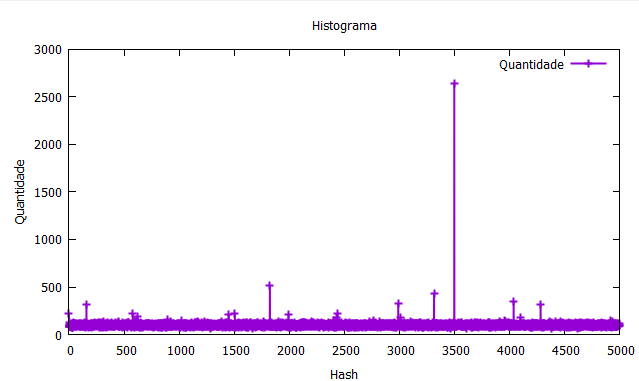
\includegraphics{hash_horner.png}
\end{center}
Para entendermos devemos levar em consideração que utilizamos 5000 buckets, pois o arquivo de entrada tem 1.000.000.000 de registros e foi dado no enunciado que cada bucket tem 200 itens de tamanho máximo, logo são necessários 5000 buckets para distribuir igualmente todos os registros. 

Assim podemos observar que de fato a maioria dos buckets não teve mais de 200 itens, apenas alguns estouraram sendo necessário usar buckets de estouro para poder atende-los. além disso pelo gráfico podemos observar que a função de fato aparenta ter distribuição uniforme. Os buckets com valores muito maiores podem, provavelmente, atender registros com aparições mais frequentes do que os demais. 

\begin{thebibliography}{00}
	\bibitem{Fontes}
	UCSD, Hash functions for strings.
	disponível em \url{https://cseweb.ucsd.edu/~kube/cls/100/Lectures/lec16/lec16-12.html}
\end{thebibliography}

    
\end{document}


